\documentclass[12pt,a4paper]{report}

% ── Packages ──────────────────────────────────────────────────
\usepackage[utf8]{inputenc}
\usepackage[T1]{fontenc}
\usepackage[french]{babel}
\usepackage{geometry}
\usepackage{graphicx}
\usepackage{xcolor}
\usepackage{hyperref}
\usepackage{fancyhdr}
\usepackage{titlesec}
\usepackage{booktabs}
\usepackage{array}
\usepackage{enumitem}
\usepackage{listings}
\usepackage{tcolorbox}
\usepackage{float}
\usepackage{subcaption}
\usepackage{fontawesome5}
\usepackage{mdframed}
\usepackage{lmodern}
\usepackage{microtype}
\usepackage{setspace}

\geometry{left=2.5cm, right=2.5cm, top=3cm, bottom=3cm}

% ── Couleurs OCP ──────────────────────────────────────────────
\definecolor{ocpGreen}{RGB}{0,132,61}
\definecolor{ocpGold}{RGB}{196,118,10}
\definecolor{ocpDark}{RGB}{28,26,20}
\definecolor{ocpLight}{RGB}{247,242,230}
\definecolor{ocpBlue}{RGB}{41,128,185}
\definecolor{codebg}{RGB}{245,245,245}

% ── Hyperref ──────────────────────────────────────────────────
\hypersetup{
  colorlinks=true,
  linkcolor=ocpGreen,
  urlcolor=ocpBlue,
  citecolor=ocpGold,
  pdftitle={MineAssist -- Rapport Technique PFE},
  pdfauthor={Youness Bilouche},
}

% ── En-têtes / pieds de page ──────────────────────────────────
\pagestyle{fancy}
\fancyhf{}
\fancyhead[L]{\textcolor{ocpGreen}{\textbf{MineAssist}} \textcolor{ocpGold}{|} Rapport PFE}
\fancyhead[R]{\textcolor{gray}{\small OCP -- CAT 994F}}
\fancyfoot[C]{\thepage}
\renewcommand{\headrulewidth}{0.5pt}
\renewcommand{\headrule}{\hbox to\headwidth{\color{ocpGreen}\leaders\hrule height \headrulewidth\hfill}}

% ── Styles titres ─────────────────────────────────────────────
\titleformat{\chapter}[block]
  {\huge\bfseries\color{ocpGreen}}
  {\thechapter.}{12pt}{}
  [\vspace{2pt}\color{ocpGold}\hrule height 2pt]

\titleformat{\section}
  {\Large\bfseries\color{ocpDark}}
  {\thesection}{8pt}{}

\titleformat{\subsection}
  {\large\bfseries\color{ocpGreen!80!black}}
  {\thesubsection}{6pt}{}

% ── Listing code ──────────────────────────────────────────────
\lstset{
  backgroundcolor=\color{codebg},
  basicstyle=\ttfamily\small,
  breaklines=true,
  frame=single,
  rulecolor=\color{ocpGold!50},
  keywordstyle=\color{ocpGreen}\bfseries,
  commentstyle=\color{gray}\itshape,
  numbers=left,
  numberstyle=\tiny\color{gray},
}

% ── Boîte info ────────────────────────────────────────────────
\tcbuselibrary{skins,breakable}
\newtcolorbox{infobox}[1]{
  colback=ocpLight,
  colframe=ocpGreen,
  fonttitle=\bfseries\color{white},
  title=#1,
  coltitle=white,
  boxrule=1pt,
}

\setstretch{1.2}

% ═══════════════════════════════════════════════════════════════
\begin{document}
% ═══════════════════════════════════════════════════════════════

% ── Page de titre ─────────────────────────────────────────────
\begin{titlepage}
  \pagecolor{ocpDark}
  \color{white}
  \centering
  \vspace*{2cm}

  % Logo OCP simulé
  \begin{tcolorbox}[
    colback=ocpGreen, colframe=ocpGold, boxrule=2pt,
    width=5cm, halign=center, valign=center, height=1.5cm
  ]
    {\Huge\bfseries\texttt{OCP}}
  \end{tcolorbox}

  \vspace{1cm}
  {\color{ocpGold}\hrule height 1pt}
  \vspace{0.5cm}

  {\fontsize{38}{46}\selectfont\bfseries\textcolor{ocpGreen}{MineAssist}}\\[0.3cm]
  {\Large\textcolor{ocpGold}{Plateforme Intelligente de Maintenance Prédictive}}\\[0.2cm]
  {\large\textcolor{gray}{CAT 994F -- OCP Benguérir -- Site Phosphate}}

  \vspace{1cm}
  {\color{ocpGold}\hrule height 1pt}
  \vspace{1.5cm}

  \begin{tcolorbox}[colback=ocpDark!80, colframe=ocpGold, boxrule=1pt]
    \centering
    {\large\bfseries Rapport de Projet de Fin d'Études}\\[0.4cm]
    \begin{tabular}{ll}
      \textcolor{ocpGold}{Auteur :}      & Youness Bilouche \\[4pt]
      \textcolor{ocpGold}{Encadrant :}   & [Nom Encadrant] \\[4pt]
      \textcolor{ocpGold}{Établissement :} & [Votre École] \\[4pt]
      \textcolor{ocpGold}{Année :}       & 2025 -- 2026 \\[4pt]
      \textcolor{ocpGold}{Version :}     & v2.0 (Mai 2026) \\
    \end{tabular}
  \end{tcolorbox}

  \vfill
  {\small\textcolor{gray}{Confidentiel -- Usage interne OCP}}
\end{titlepage}

\pagecolor{white}\color{black}

% ── Résumé ────────────────────────────────────────────────────
\chapter*{Résumé}
\addcontentsline{toc}{chapter}{Résumé}

\begin{infobox}{MineAssist en bref}
MineAssist est une plateforme web full-stack de \textbf{maintenance prédictive} et de \textbf{diagnostic assisté par IA}
dédiée aux chargeuses sur pneus \textbf{CAT 994F} opérant sur le site de phosphate d'OCP Benguérir (Maroc).
\end{infobox}

\vspace{1em}
La plateforme intègre :
\begin{itemize}[leftmargin=1.5cm]
  \item Un \textbf{moteur RAG} (Retrieval-Augmented Generation) basé sur la documentation technique CAT 994F
  \item Un système de \textbf{diagnostic de pannes} avec décodage automatique des codes MID/CID/FMI et VIMS
  \item Des \textbf{modèles ML} (XGBoost, Random Forest, Isolation Forest) pour la détection d'anomalies
  \item Un \textbf{dashboard exécutif} unifié avec KPIs temps réel
  \item Une \textbf{analyse d'huile} complète (VHVI, usure, contamination)
  \item Un système \textbf{multi-agents} pour le conseil d'experts virtuels
\end{itemize}

\vspace{1em}
\textbf{Technologies :} React 18 + Vite (frontend), FastAPI + Python 3.11 (backend), ChromaDB (RAG), OpenRouter LLM, Docker, GitHub Actions CI/CD.

\clearpage

% ── Table des matières ────────────────────────────────────────
\tableofcontents
\clearpage

% ══════════════════════════════════════════════════════════════
\chapter{Introduction et Contexte}
% ══════════════════════════════════════════════════════════════

\section{Contexte industriel}

L'Office Chérifien des Phosphates (\textbf{OCP}) est le leader mondial de l'industrie du phosphate,
opérant sur plusieurs sites miniers au Maroc. Sur le site de \textbf{Benguérir}, les chargeuses
sur pneus \textbf{CAT 994F} constituent l'épine dorsale de l'extraction, chargement et
transport du minerai.

Chaque engin représente un investissement de plusieurs millions de dollars et une immobilisation
non planifiée entraîne des pertes de production considérables. Dans ce contexte, la transition
d'une maintenance \emph{corrective} vers une maintenance \emph{prédictive} est devenue
une priorité stratégique.

\section{Problématique}

Les équipes de maintenance font face à plusieurs défis :

\begin{itemize}
  \item \textbf{Volume de données :} les CAT 994F génèrent des milliers de paramètres VIMS
  (codes MID/CID/FMI, températures, pressions, vibrations)
  \item \textbf{Dispersion documentaire :} la documentation technique (CHF442, RENR6306,
  RENR9347) est volumineuse et difficile à consulter rapidement
  \item \textbf{Expertise centralisée :} le diagnostic de pannes complexes requiert
  des spécialistes rares
  \item \textbf{Réactivité :} le délai entre détection d'anomalie et intervention
  reste trop long
\end{itemize}

\section{Objectifs du projet}

MineAssist vise à :
\begin{enumerate}
  \item Centraliser et rendre interrogeable l'ensemble de la documentation technique via une IA
  \item Automatiser le décodage des codes défauts et proposer des procédures de diagnostic
  \item Prédire les défaillances avant qu'elles n'impactent la production
  \item Fournir un tableau de bord unifié pour les équipes de maintenance et la direction
\end{enumerate}

% ══════════════════════════════════════════════════════════════
\chapter{Architecture Technique}
% ══════════════════════════════════════════════════════════════

\section{Vue d'ensemble}

MineAssist suit une architecture \textbf{microservices} découplée en deux couches principales :

\begin{center}
\begin{tcolorbox}[colback=ocpLight, colframe=ocpGreen, width=0.9\textwidth]
\centering
\textbf{Frontend React (Vite)} $\xrightarrow{\text{HTTP/REST}}$ \textbf{Backend FastAPI} $\xrightarrow{}$ \textbf{ChromaDB + LLM}\\[8pt]
\small{Port 5173 \hspace{4cm} Port 8000 \hspace{2cm} OpenRouter API}
\end{tcolorbox}
\end{center}

\section{Stack technologique}

\begin{table}[H]
\centering
\begin{tabular}{>{\bfseries}p{3cm} p{5cm} p{5cm}}
\toprule
\textcolor{ocpGreen}{Couche} & \textcolor{ocpGreen}{Technologies} & \textcolor{ocpGreen}{Rôle} \\
\midrule
Frontend & React 18, Vite, CSS-in-JS & Interface utilisateur SPA \\
\addlinespace
Backend & FastAPI, Python 3.11, Pydantic & API REST, logique métier \\
\addlinespace
IA / RAG & ChromaDB, OpenRouter, LLaMA 3.3 70B & Moteur de réponses \\
\addlinespace
ML & XGBoost, Random Forest, Isolation Forest & Prédiction, anomalies \\
\addlinespace
Auth & JWT, bcrypt & Authentification sécurisée \\
\addlinespace
DevOps & Docker, GitHub Actions, Nginx & CI/CD, déploiement \\
\bottomrule
\end{tabular}
\caption{Stack technologique de MineAssist}
\end{table}

\section{Architecture Backend}

Le backend FastAPI expose \textbf{96+ routes} organisées en modules :

\begin{itemize}
  \item \texttt{/ask} \& \texttt{/ask/v2} -- Questions libres via RAG + LLM
  \item \texttt{/diagnose} \& \texttt{/diagnose/v2} -- Diagnostic structuré de pannes
  \item \texttt{/pred/*} -- Prédictions XGBoost / Random Forest
  \item \texttt{/ml/*} -- Score de santé, détection d'anomalies
  \item \texttt{/gmao/*} -- Analytics GMAO (anomalies, capteurs, géo)
  \item \texttt{/oil/*} -- Analyse d'huile
  \item \texttt{/auth/*} -- Authentification JWT
  \item \texttt{/notifications/*} -- Alertes en temps réel
  \item \texttt{/metrics} -- Métriques Prometheus
\end{itemize}

\section{Moteur RAG (Retrieval-Augmented Generation)}

Le cœur du système de Q\&R documentaire est basé sur :

\begin{enumerate}
  \item \textbf{Indexation} : Les documents techniques (PDF, PPTX) sont découpés en chunks
  et vectorisés via un modèle d'embeddings
  \item \textbf{Stockage} : Les vecteurs sont stockés dans ChromaDB avec fallback lexical
  \item \textbf{Récupération} : Pour chaque question, les $k$ chunks les plus pertinents
  sont extraits
  \item \textbf{Génération} : Le contexte + la question sont envoyés au LLM
  (LLaMA 3.3 70B via OpenRouter)
\end{enumerate}

% ══════════════════════════════════════════════════════════════
\chapter{Fonctionnalités et Captures d'Écran}
% ══════════════════════════════════════════════════════════════

\section{Page de Connexion}

La page de connexion adopte l'identité visuelle OCP avec fond sombre, logo et animations
d'entrée. L'authentification est sécurisée par JWT avec gestion des rôles (admin, opérateur).

\begin{figure}[H]
  \centering
  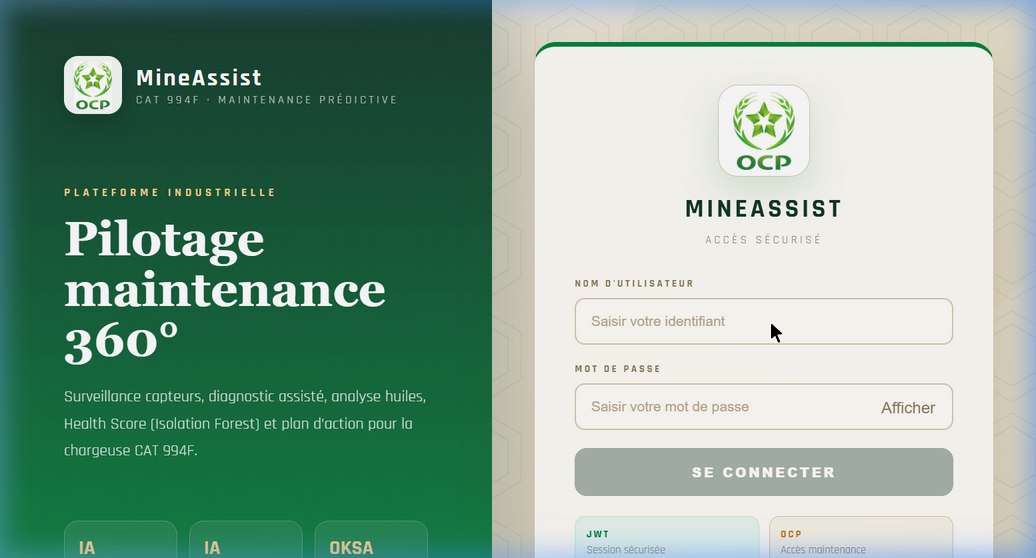
\includegraphics[width=0.85\textwidth]{images/screen1.png}
  \caption{Page de connexion sécurisée MineAssist}
\end{figure}

\section{Dashboard Exécutif 360°}

Le tableau de bord principal offre une vue consolidée de l'état de flotte :

\begin{itemize}
  \item KPIs en temps réel (disponibilité, score de santé, alertes actives)
  \item Graphiques de tendance (anomalies par mois, répartition par sous-système)
  \item Navigation rapide vers tous les modules
\end{itemize}

\begin{figure}[H]
  \centering
  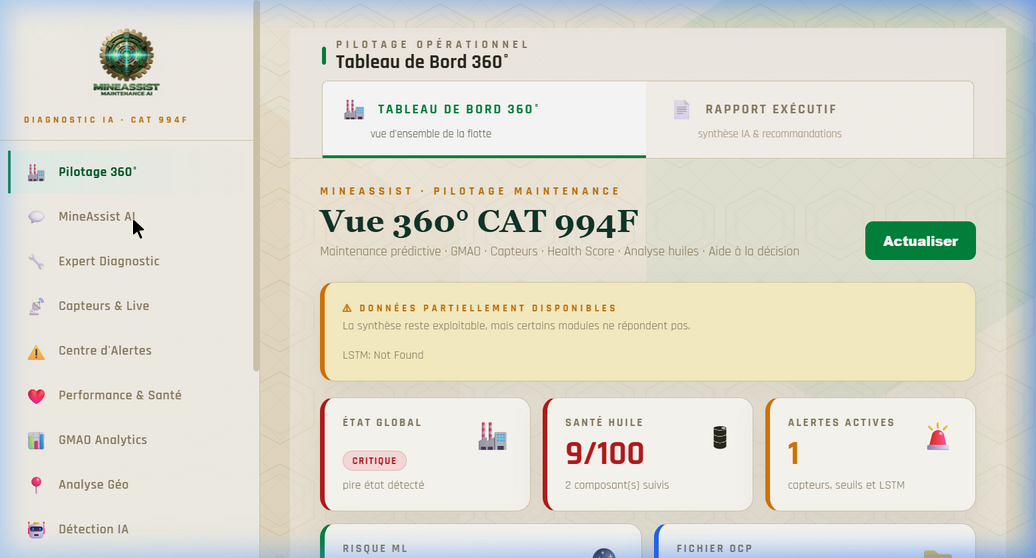
\includegraphics[width=0.9\textwidth]{images/screen3.png}
  \caption{Dashboard Exécutif 360° -- Vue globale de la flotte}
\end{figure}

\section{MineAssist AI -- Question-Réponse Documentaire}

Le module Q\&R permet aux techniciens d'interroger en langage naturel
l'ensemble de la documentation technique CAT 994F (CHF442, RENR6306, RENR9347,
schémas hydrauliques et électriques).

\begin{figure}[H]
  \centering
  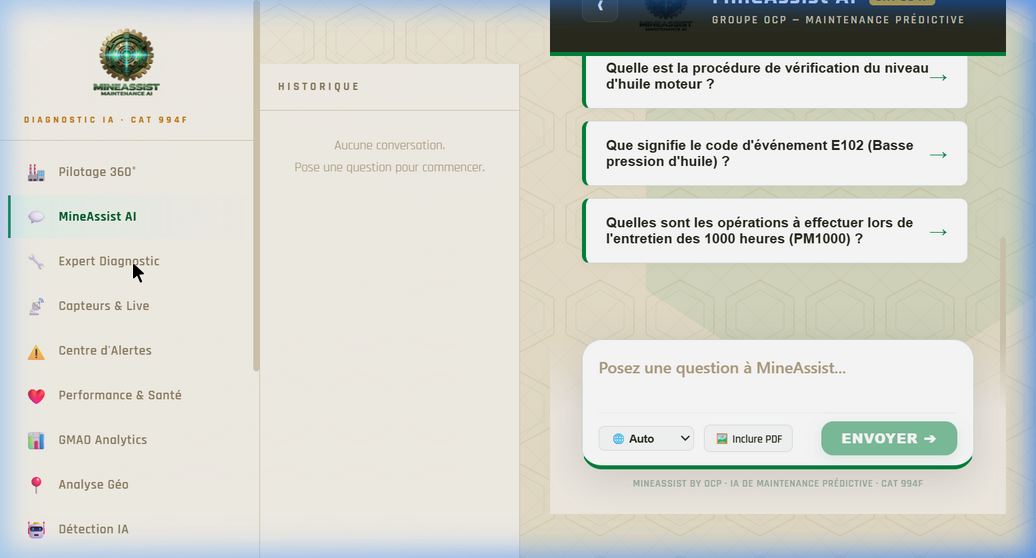
\includegraphics[width=0.9\textwidth]{images/screen4.png}
  \caption{Interface MineAssist AI -- Interrogation documentaire en langage naturel}
\end{figure}

\subsection{Fonctionnalités avancées}
\begin{itemize}
  \item \textbf{Sources citées} : chaque réponse indique les documents sources
  \item \textbf{Illustrations extraites} : les pages PDF pertinentes sont affichées
  \item \textbf{Localisation dans les schémas} : mise en évidence automatique
  des composants sur les schémas hydrauliques/électriques
  \item \textbf{Streaming} : réponse en temps réel (endpoint \texttt{/ask/stream})
\end{itemize}

\section{Expert Diagnostic -- Décodeur de Pannes}

Le module de diagnostic est l'outil central pour les techniciens de terrain.
Il intègre un décodeur instantané des codes défaut CAT 994F.

\begin{figure}[H]
  \centering
  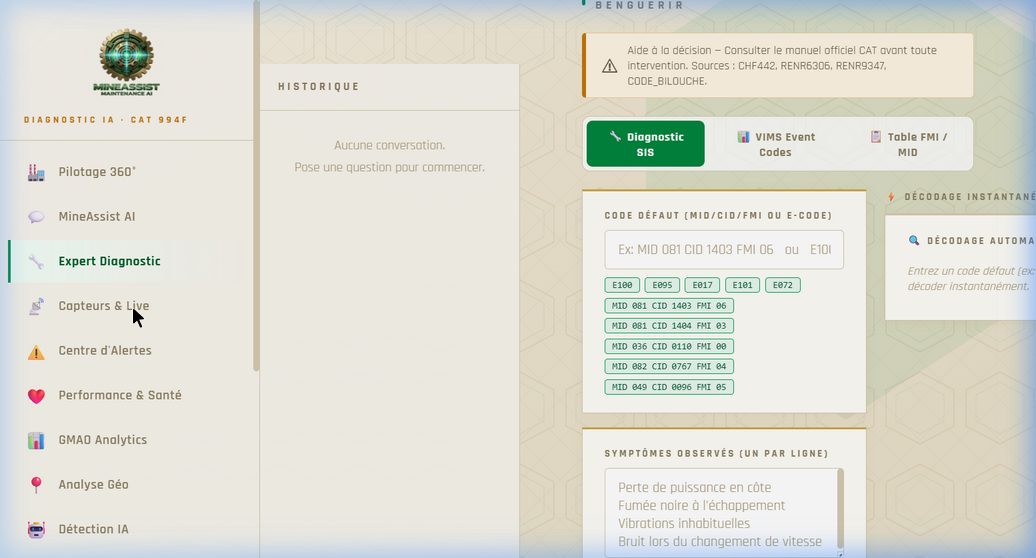
\includegraphics[width=0.9\textwidth]{images/screen5.png}
  \caption{Module Expert Diagnostic avec décodeur MID/CID/FMI}
\end{figure}

\subsection{Base de données intégrée}
Le décodeur couvre :
\begin{itemize}
  \item \textbf{MID 036} (ECM Moteur) -- 20+ composants
  \item \textbf{MID 081} (TCM Transmission) -- 25+ solénoïdes et capteurs
  \item \textbf{MID 082} (Impléments hydrauliques) -- 15+ composants
  \item \textbf{MID 049} (VIMS) -- 12+ capteurs de surveillance
  \item \textbf{19 codes FMI} avec procédures de diagnostic détaillées
  \item \textbf{18 VIMS Event Codes} (E017 à E2089)
\end{itemize}

\begin{figure}[H]
  \centering
  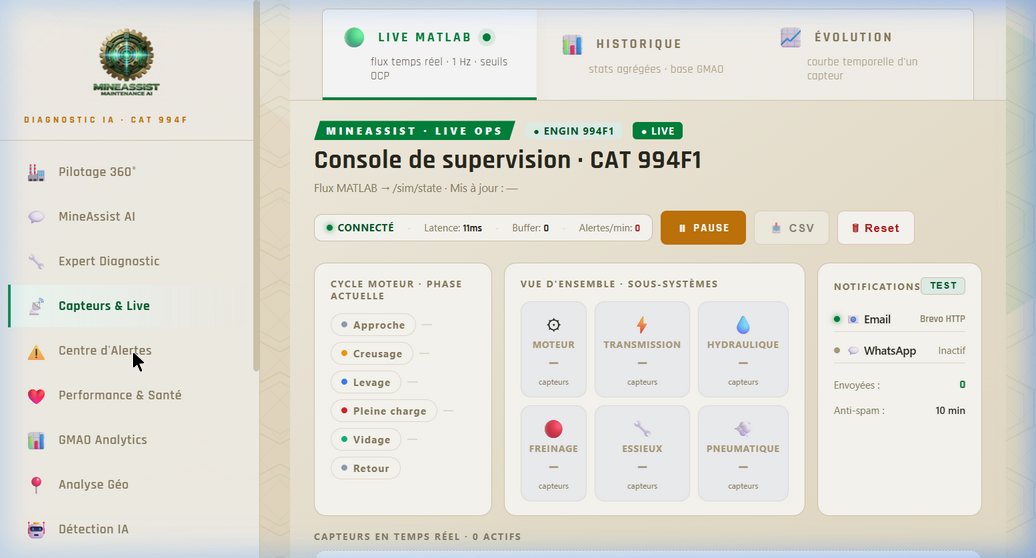
\includegraphics[width=0.9\textwidth]{images/screen6.png}
  \caption{Résultat de diagnostic LLM structuré avec rendu DiagnosticRenderer}
\end{figure}

\section{Capteurs \& Monitoring Live}

Visualisation en temps réel des paramètres capteurs issus des fichiers GMAO :
températures, pressions, vitesses, avec détection des dépassements de seuils.

\begin{figure}[H]
  \centering
  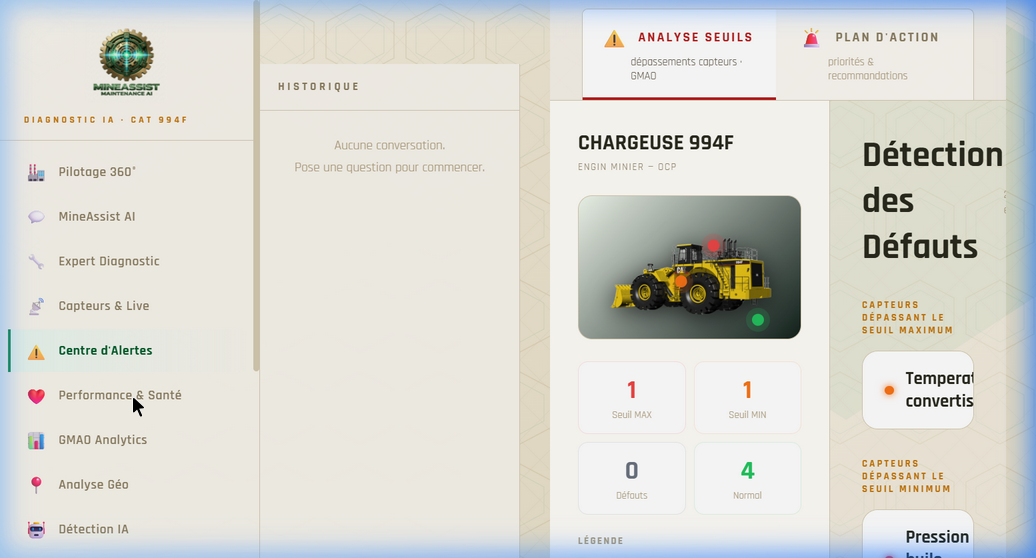
\includegraphics[width=0.9\textwidth]{images/screen7.png}
  \caption{Page Capteurs \& Live -- Monitoring des paramètres temps réel}
\end{figure}

\section{Centre d'Alertes OCP}

Centralisation et priorisation des alertes actives par gravité (G1 à G3),
avec filtrage par machine, sous-système et période.

\begin{figure}[H]
  \centering
  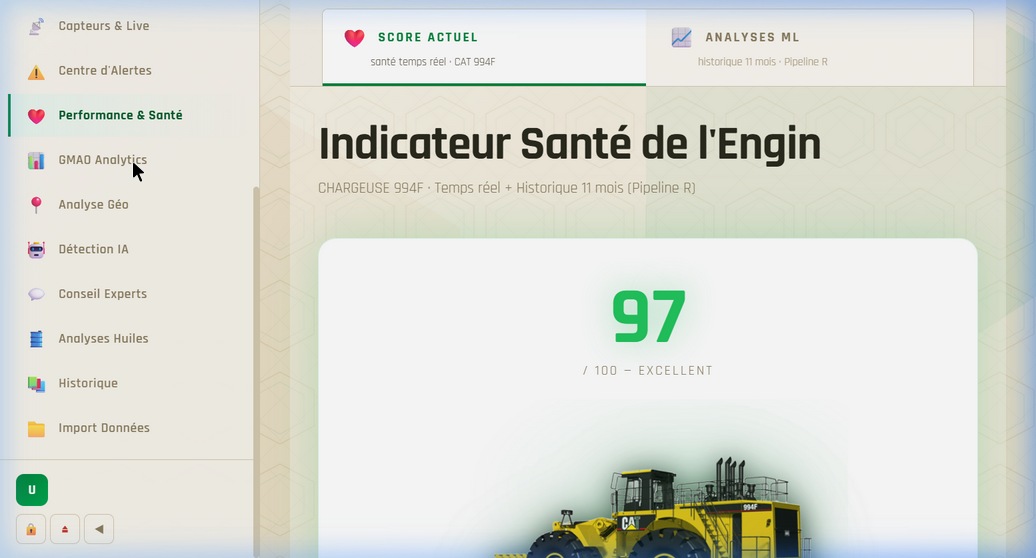
\includegraphics[width=0.9\textwidth]{images/screen8.png}
  \caption{Centre d'Alertes -- Tableau de bord des alertes actives}
\end{figure}

\section{Performance \& Santé Machine}

Score de santé ML calculé par modèle Random Forest, historique des pannes,
RUL (Remaining Useful Life) estimé par sous-système.

\begin{figure}[H]
  \centering
  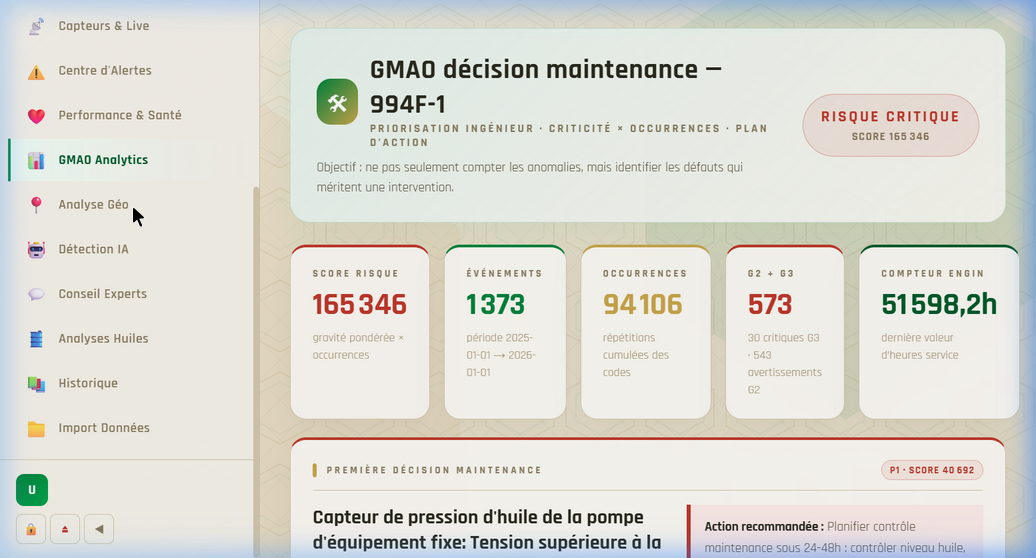
\includegraphics[width=0.9\textwidth]{images/screen9.png}
  \caption{Performance \& Santé -- Score ML et RUL par sous-système}
\end{figure}

\section{GMAO Analytics}

Analyse statistique des données GMAO : répartition des anomalies par mois,
par code défaut, par gravité, avec calcul de score de risque pondéré.

\begin{figure}[H]
  \centering
  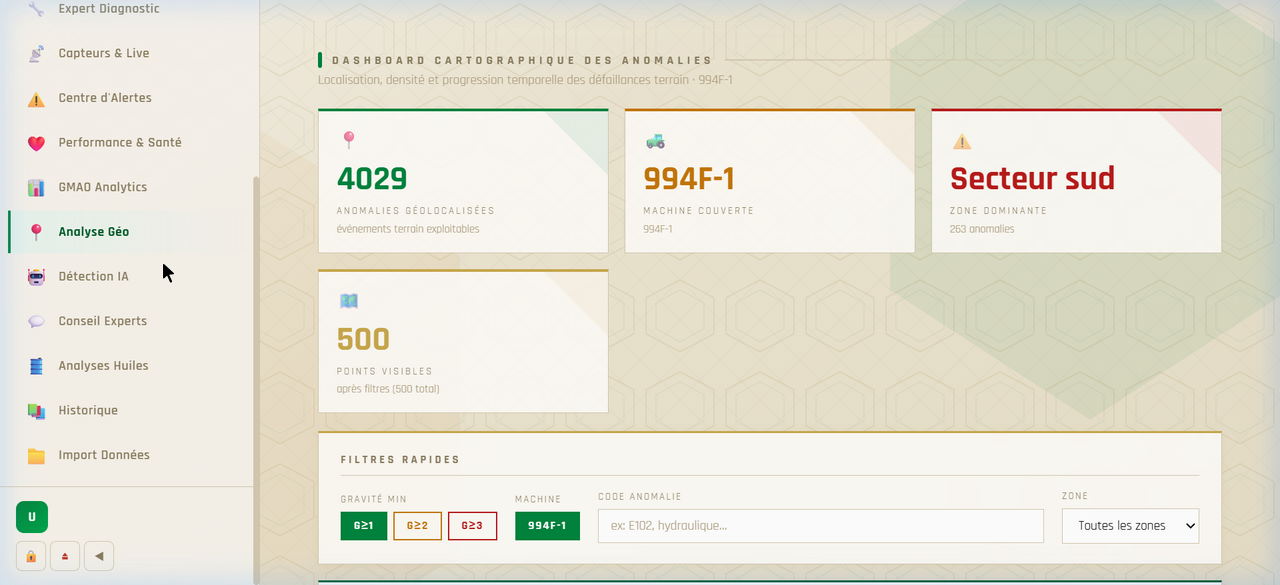
\includegraphics[width=0.9\textwidth]{images/screen10.png}
  \caption{GMAO Analytics -- Analyse historique des anomalies}
\end{figure}

\section{Analyse Géospatiale}

Cartographie des anomalies sur le site minier avec segmentation automatique
en zones (nord, sud, chargement, circulation, rampe) et identification
des zones à risque prioritaire.

\begin{figure}[H]
  \centering
  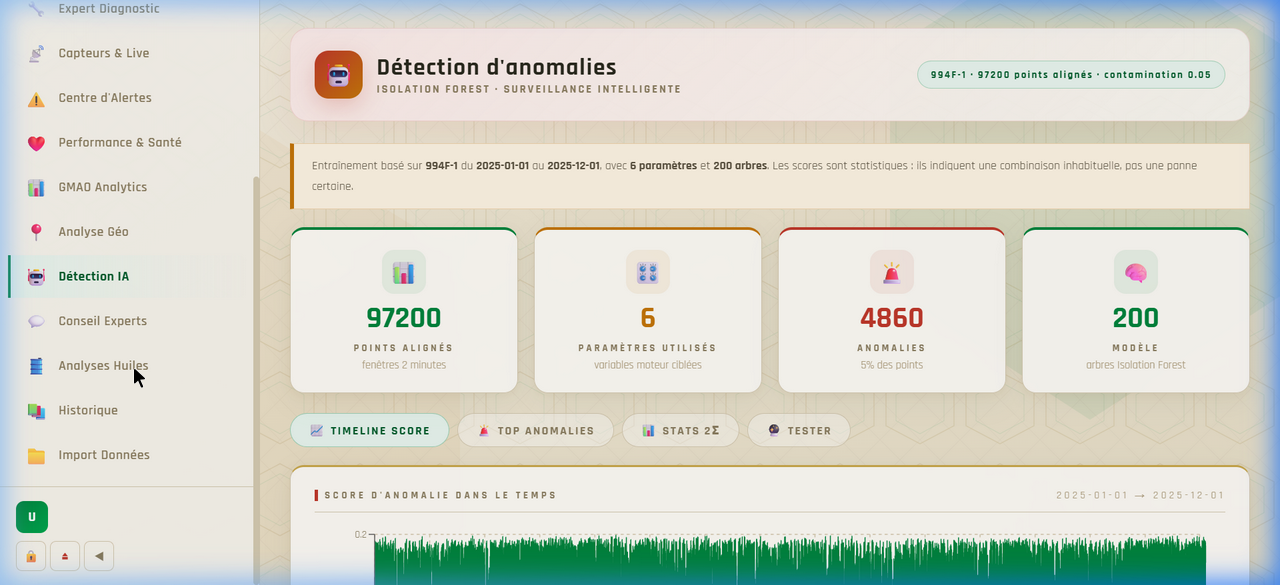
\includegraphics[width=0.9\textwidth]{images/screen11.png}
  \caption{Analyse Géo -- Cartographie spatiale des anomalies sur site}
\end{figure}

\section{Détection d'Anomalies par IA}

Modèle \textbf{Isolation Forest} entraîné sur les données capteurs GMAO pour
détecter les comportements anormaux sans étiquetage (apprentissage non supervisé).

\begin{figure}[H]
  \centering
  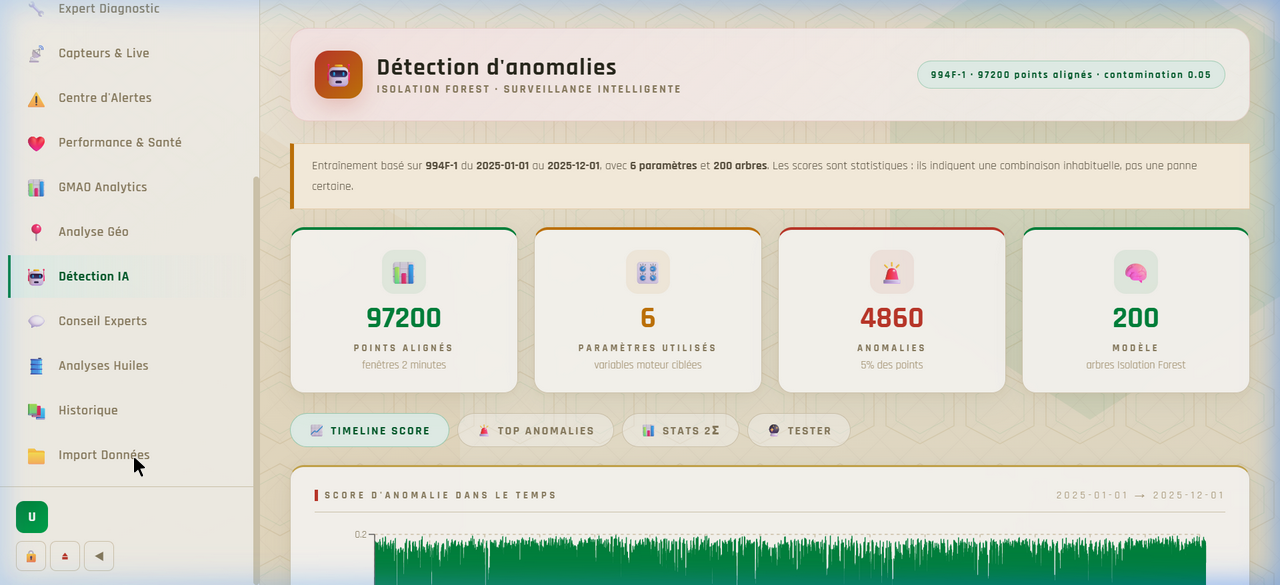
\includegraphics[width=0.9\textwidth]{images/screen12.png}
  \caption{Détection IA -- Anomalies détectées par Isolation Forest}
\end{figure}

\section{Analyses d'Huile}

Module dédié à l'interprétation des analyses d'huile : viscosité VHVI,
particules d'usure (Fe, Cu, Pb), contamination eau/carburant,
avec recommandations automatiques basées sur les seuils OCP.

\section{Import de Données OCP}

Interface de gestion des fichiers GMAO : upload des fichiers Excel/CSV
d'anomalies et de capteurs, avec validation et résumé statistique automatique.

% ══════════════════════════════════════════════════════════════
\chapter{Modèles Machine Learning}
% ══════════════════════════════════════════════════════════════

\section{Architecture du Pipeline ML}

Le backend intègre un pipeline Machine Learning complet pour l'analyse prédictive et la détection d'anomalies, entraîné sur l'historique GMAO et les séries temporelles des capteurs. La persistance des modèles et des transformateurs est assurée via \texttt{joblib} (format \texttt{.pkl}).

\subsection{Préparation des données (Preprocessing)}
Avant l'inférence, les données subissent plusieurs étapes de transformation mathématique :
\begin{itemize}
  \item \textbf{Imputation des valeurs manquantes} : Utilisation des modèles \texttt{imputer.pkl}, \texttt{imputer\_rf.pkl} et \texttt{imputer\_if.pkl} pour traiter dynamiquement les données aberrantes ou les pertes de communication des capteurs.
  \item \textbf{Normalisation} : Application d'un algorithme \texttt{StandardScaler} via des objets dédiés (\texttt{scaler.pkl}, \texttt{scaler\_rf.pkl}, \texttt{scaler\_if.pkl}) pour standardiser les échelles des signaux de pressions et de températures avant leur traitement.
\end{itemize}

\section{Modèles Déployés}

La plateforme s'appuie sur une combinaison hybride de modèles supervisés et non supervisés pour couvrir de manière holistique les besoins de maintenance prédictive.

\begin{table}[H]
\centering
\begin{tabular}{>{\bfseries}p{3cm} p{4cm} p{7cm}}
\toprule
\textcolor{ocpGreen}{Modèle} & \textcolor{ocpGreen}{Technique} & \textcolor{ocpGreen}{Application et Objectif} \\
\midrule
Isolation Forest & Non supervisé (Détection) & Détection précoce de comportements atypiques multidimensionnels sur les flux VIMS (\texttt{isolation\_forest.pkl}). \\
\addlinespace
Random Forest & Supervisé (Classification) & Modèle ensembliste évaluant la gravité des défauts (G1 à G3) et générant le score de santé global (\texttt{random\_forest\_gravite.pkl}). \\
\addlinespace
XGBoost & Supervisé (Classification) & Détection des alertes critiques et prédiction des seuils de criticité via apprentissage par boosting (\texttt{xgboost\_alerte.pkl}). \\
\addlinespace
Gradient Boosting & Supervisé (Ensemble) & Modèle alternatif optimisé pour la validation et l'anticipation d'alertes (\texttt{gradient\_boosting\_alerte.pkl}). \\
\addlinespace
K-Means & Non supervisé (Clustering) & Identification automatique des régimes de fonctionnement de l'engin (ex: ralenti, charge, levage) (\texttt{kmeans\_modes.pkl}). \\
\bottomrule
\end{tabular}
\caption{Cartographie des modèles ML intégrés dans l'écosystème MineAssist}
\end{table}

\section{Ingénierie des Features et Évaluation}

\subsection{Espace Vectoriel (Feature Engineering)}
Le dictionnaire \texttt{feature\_names.json} gère dynamiquement l'alignement des tenseurs d'entrée. L'apprentissage s'est concentré sur des caractéristiques physiques clés :
\begin{itemize}
  \item \textbf{Télémétrie Moteur (MID 036)} : Régime de rotation, delta de pression d'huile filtrée/non-filtrée, températures des collecteurs d'échappement.
  \item \textbf{Cinématique (MID 081)} : Température de l'huile du convertisseur de couple (TC), régime de sortie de transmission, pressions d'embrayage (CL1-CL5).
  \item \textbf{Hydraulique (MID 082)} : Haute pression de la pompe d'implément et charge hydraulique.
  \item \textbf{Méta-features temporelles} : Dérivées premières des signaux (vélocité de changement), moyennes mobiles, et accumulation des heures de service.
\end{itemize}

\subsection{Monitoring MLOps}
L'historique des cycles d'entraînement croisés est tracé en continu dans \texttt{train\_results.csv}, offrant une traçabilité sur l'évolution des métriques (Accuracy, F1-Score, RMSE) face à la dérive potentielle des données (Data Drift). L'endpoint backend \texttt{/metrics} expose ces KPI en temps réel pour Prometheus.

\section{Système Multi-Agents Cognitifs (SMA)}

En complément des approches quantitatives classiques, une couche de raisonnement symbolique par \textbf{Système Multi-Agents (SMA)} agit comme comité d'experts virtuels :

\begin{itemize}
  \item \textbf{Agent Moteur} : Spécialiste de la thermodynamique, de l'injection et du refroidissement (ECM).
  \item \textbf{Agent Transmission} : Expert du transfert de puissance, des embrayages et de la gestion TCM.
  \item \textbf{Agent Hydraulique} : Spécialiste des pressions et de l'activation des vérins et pompes.
  \item \textbf{Agent VIMS} : Analyste de la logique système et des matrices Event Codes.
\end{itemize}

Lorsqu'une anomalie complexe est détectée, l'\textbf{Agent Coordinateur} distribue l'investigation aux agents de spécialité. Ces derniers fusionnent l'état ML (scores, probabilités) avec la base documentaire RAG pour formuler un diagnostic final argumenté, proche de l'analyse d'un ingénieur fiabiliste senior.

% ══════════════════════════════════════════════════════════════
\chapter{Sécurité et Déploiement}
% ══════════════════════════════════════════════════════════════

\section{Sécurité}

\begin{itemize}
  \item \textbf{Authentification JWT} avec expiration configurable
  \item \textbf{Hachage bcrypt} des mots de passe (coût 12)
  \item \textbf{CORS} configuré par variable d'environnement
  \item \textbf{Gestion des rôles} : admin, opérateur, lecteur
  \item \textbf{Changement de mot de passe} depuis l'interface
\end{itemize}

\section{CI/CD avec GitHub Actions}

Le pipeline CI/CD automatisé comprend 3 jobs :

\begin{enumerate}
  \item \textbf{Backend} : lint (ruff), smoke test, pytest
  \item \textbf{Frontend} : lint (ESLint), build (Vite), upload artifact
  \item \textbf{Docker} : build des images backend et frontend (sur push main uniquement)
\end{enumerate}

\section{Architecture Docker}

\begin{lstlisting}[language=bash, caption={Structure Docker du projet}]
AI_994F_Assistant/
├── backend/
│   └── Dockerfile          # Python 3.11-slim + uvicorn
├── frontend/
│   └── Dockerfile          # Node 20 build + Nginx serve
└── docker-compose.yml      # Orchestration complète
\end{lstlisting}

% ══════════════════════════════════════════════════════════════
\chapter{Conclusion et Perspectives}
% ══════════════════════════════════════════════════════════════

\section{Bilan}

MineAssist constitue une solution complète et opérationnelle de maintenance prédictive
adaptée aux contraintes industrielles d'OCP. Le projet démontre la faisabilité
d'intégrer des technologies d'IA avancées (LLM, RAG, ML) dans un contexte de
maintenance industrielle critique.

\subsection*{Résultats clés}
\begin{itemize}
  \item \textbf{96+ endpoints API} couvrant tous les besoins fonctionnels
  \item \textbf{Base documentaire complète} : CHF442, RENR6306, RENR9347, schémas
  \item \textbf{3 modèles ML} entraînés sur données réelles GMAO
  \item \textbf{Temps de réponse diagnostic} : $<$ 3 secondes (décodage local)
  \item \textbf{Architecture scalable} : Docker + GitHub Actions CI/CD
\end{itemize}

\section{Perspectives}

\begin{enumerate}
  \item \textbf{Extension multi-engins} : CAT 992, Komatsu PC8000
  \item \textbf{Connectivité VIMS direct} : intégration temps réel via OBD/CAN
  \item \textbf{Application mobile} : version React Native pour techniciens terrain
  \item \textbf{Modèles spécialisés} : fine-tuning LLM sur corpus technique CAT
  \item \textbf{Digital Twin} : simulation 3D de l'engin pour formation
\end{enumerate}

\vspace{2cm}

\begin{center}
\begin{tcolorbox}[colback=ocpLight, colframe=ocpGreen, width=0.7\textwidth, halign=center]
  \textbf{\Large MineAssist v2.0}\\[4pt]
  \textcolor{ocpGold}{``L'IA au service de la mine de demain''}\\[4pt]
  \small OCP Group -- Site de Benguérir -- 2026
\end{tcolorbox}
\end{center}

% ── Bibliographie ─────────────────────────────────────────────
\chapter*{Références}
\addcontentsline{toc}{chapter}{Références}

\begin{enumerate}
  \item Caterpillar Inc., \textit{CAT 994F Electrical System Schematic} (CHF442), 2018.
  \item Caterpillar Inc., \textit{RENR6306 -- Electronic Transmission Control}, 2017.
  \item Caterpillar Inc., \textit{RENR9347 -- Engine Electronic Control System}, 2019.
  \item Caterpillar Inc., \textit{RENR6318 -- VIMS (Vital Information Management System)}, 2017.
  \item Lewis, J. et al., \textit{Retrieval-Augmented Generation for Knowledge-Intensive NLP Tasks}, NeurIPS, 2020.
  \item Chen, T., Guestrin, C., \textit{XGBoost: A Scalable Tree Boosting System}, KDD, 2016.
  \item Liu, F., Ting, K., Zhou, Z., \textit{Isolation Forest}, ICDM, 2008.
  \item FastAPI Documentation, \url{https://fastapi.tiangolo.com}
  \item React Documentation, \url{https://react.dev}
  \item ChromaDB Documentation, \url{https://docs.trychroma.com}
\end{enumerate}

\end{document}
